\documentclass[11pt,a4paper]{article}
\usepackage[utf8]{inputenc}
\usepackage{natbib}
\usepackage{authblk}

%\VignetteIndexEntry{Learning how to use the indicspecies package}
%\VignettePackage{indicspecies}

\title{How to use the \texttt{indicspecies} package (ver. 1.7.7)}
\author[1]{Miquel De Cáceres}
\affil[1]{CTFC - Forest Sciences and Technology Center of Catalonia, Spain}

\usepackage{Sweave}
\begin{document}
\Sconcordance{concordance:indicspeciesTutorial.tex:indicspeciesTutorial.Rnw:%
1 12 1 1 0 4 1 1 4 5 1 1 2 4 0 1 2 4 1 1 2 4 0 1 2 3 1 1 2 %
1 0 1 1 7 0 2 2 1 0 2 1 9 0 1 2 8 1 1 3 5 0 1 2 4 1 1 2 42 %
0 1 2 5 1 1 2 42 0 1 2 3 1 1 2 64 0 2 2 40 0 1 2 3 1 1 2 1 %
0 1 2 4 0 1 2 2 1 1 3 5 0 1 2 3 1 1 2 44 0 1 2 2 1 1 2 13 0 %
2 2 13 0 1 2 7 1 1 3 2 0 1 1 36 0 1 2 2 1 1 3 2 0 1 1 41 0 %
1 2 5 1 1 3 2 0 1 1 37 0 2 2 40 0 1 2 5 1 1 2 1 0 1 1 12 0 %
1 2 1 3 2 0 1 1 11 0 1 1 12 0 1 2 4 1 1 3 2 0 1 1 12 0 1 2 %
5 1 1 2 8 0 1 2 2 1 1 2 8 0 1 2 5 1 1 2 1 0 2 1 1 3 6 0 1 2 %
9 1 1 2 1 0 1 1 6 0 1 2 1 3 2 0 1 1 70 0 1 2 3 1 1 4 48 0 2 %
2 14 0 1 2 5 1 1 2 7 0 2 2 7 0 1 2 3 1 1 2 1 0 1 1 1 2 5 0 %
1 2 4 1 1 2 12 0 1 1 9 0 1 2 3 1 1 2 4 0 2 2 4 0 2 2 4 0 2 %
2 48 0 1 2 3 1}

\maketitle
\tableofcontents

\section{Introduction}
Determining the occurrence or abundance of a small set of indicator species, as an alternative to sampling the entire community, has been particularly useful in longterm environmental monitoring for conservation or ecological management. Species are chosen as indicators if they (i) reflect the biotic or abiotic state of the environment; (ii) provide evidence for the impacts of environmental change; or (iii) predict the diversity of other species, taxa or communities within an area. 

In this tutorial we will show how to use the functions included in package \texttt{indicspecies} to conduct indicator species analysis. This package was originally created as a supplementary material to \citet{DeCaceres2009}, but has been developing since then and now \texttt{indicspecies} updates are distributed from CRAN. Before doing anything else, we need to load the functions of the package:
\begin{Schunk}
\begin{Sinput}
> library(indicspecies)
\end{Sinput}
\end{Schunk}

\section{Data required for indicator species analysis}
Indicator species are often determined using an analysis of the relationship between the species occurrence or abundance values from a set of sampled sites and the classification of the same sites into site groups, which may represent habitat types, community types, disturbance states, etc. Thus, there are two data elements in an indicator species analysis: (1) the community data matrix; and (2) the vector that describes the classification of sites into groups.
\subsection{The community data matrix}
This is a matrix (or a data frame) with sites in rows and species in columns. Normally, we will use functions like \texttt{read.table} to read our data set from a file. In this example we load our example dataset into the workspace using:
\begin{Schunk}
\begin{Sinput}
> data(wetland)
\end{Sinput}
\end{Schunk}
The wetland data set describes the vegetation of the Adelaide river alluvial plain (Australia), as sampled by \citet{Bowman1987}. It contains the abundance values of 33 species (columns) in 41 sites (rows).

\subsection{Defining the classification of sites}
In order to run an indicator species analysis we need a vector containing the classification of the sites into groups. The intepretation of these site groups is left to the user. A vector of site groups can be created, for example, using the R functions \texttt{c()} and \texttt{rep()}:
\begin{Schunk}
\begin{Sinput}
> groups = c(rep(1, 17), rep(2, 14), rep(3,10))
> groups
\end{Sinput}
\begin{Soutput}
 [1] 1 1 1 1 1 1 1 1 1 1 1 1 1 1 1 1 1 2 2 2 2 2 2 2 2 2 2 2 2 2 2
[32] 3 3 3 3 3 3 3 3 3 3
\end{Soutput}
\end{Schunk}
Alternatively, one can obtain a classification using non-hierarchical cluster analysis:
\begin{Schunk}
\begin{Sinput}
> wetkm = kmeans(wetland, centers=3)
> groupskm = wetkm$cluster
> groupskm
\end{Sinput}
\begin{Soutput}
 5  8 13  4 17  3  9 21 16 14  2 15  1  7 10 40 23 25 22 20  6 18 
 2  2  2  2  2  3  2  2  3  3  2  2  2  3  3  1  1  1  2  1  1  1 
12 39 19 11 30 34 28 31 26 29 33 24 36 37 41 27 32 35 38 
 1  1  1  1  1  1  1  1  1  1  1  1  1  1  1  1  1  2  2 
\end{Soutput}
\end{Schunk}

If the site classification vector is obtained independently of species data, the significance of statistical tests carried out on the indicator species will be meaningful. For example, one could classify the sites using environmental data before indicator species analysis. An example is found in \citet{Borcard2011}.

\section{Indicator species analysis using \texttt{multipatt}}
Function \texttt{multipatt} is the most commonly used function of \texttt{indicspecies}. It allows determining lists of species that are associated to particular groups of sites (or combinations of those). Once we have the two data components mentioned in the previous section, we are ready to run an indicator species analysis using \texttt{multipatt}.
\subsection{Indicator Value analysis with site group combinations}
When the aim is to determine which species can be used as indicators of certain site group an approach commonly used in ecology is the \emph{Indicator Value} \citep{Dufrene1997}. These authors defined an Indicator Value (IndVal) index to measure the association between a species and a site group. The method of \citet{Dufrene1997} calculates the IndVal index between the species and each site group and then looks for the group corresponding to the highest association value. Finally, the statistical significance of this relationship is tested using a permutation test. IndVal is the default index used to measure the association between a species and a group of sites in \texttt{multipatt}. However, by default \texttt{multipatt} uses an extension of the original Indicator Value method, because the function looks for indicator species of both individual site groups \emph{and} combinations of site groups, as explained in \citet{DeCaceres2010}. 

Indicator species analysis (with site group combinations) can be run using:
\begin{Schunk}
\begin{Sinput}
> indval = multipatt(wetland, groups, 
+                    control = how(nperm=999)) 
\end{Sinput}
\end{Schunk}
As mentioned before, by default \texttt{multipatt} uses the IndVal index (\texttt{func = "IndVal.g"}) as test statistic. Actually, the square root of IndVal is returned by the \texttt{multipatt} function. The option \texttt{control = how(nperm=999)} allows choosing the number of random permutations required for the permutational test (this number affects the precision of the p-value). Function \texttt{how} from the \texttt{permute} package allows defining more complex permutational designs. 

\subsubsection{Displaying the results}
When the indicator species analysis is completed, we can obtain the list of indicator species for each site group (or site group combination) using:

\begin{Schunk}
\begin{Sinput}
> summary(indval) 
\end{Sinput}
\begin{Soutput}
 Multilevel pattern analysis
 ---------------------------

 Association function: IndVal.g
 Significance level (alpha): 0.05

 Total number of species: 33
 Selected number of species: 10 
 Number of species associated to 1 group: 6 
 Number of species associated to 2 groups: 4 

 List of species associated to each combination: 

 Group 1  #sps.  3 
        stat p.value    
Ludads 0.907   0.001 ***
Orysp. 0.823   0.002 ** 
Psespi 0.602   0.019 *  

 Group 3  #sps.  3 
        stat p.value    
Pancam 0.910   0.001 ***
Eupvac 0.724   0.002 ** 
Cynarc 0.602   0.015 *  

 Group 1+2  #sps.  1 
        stat p.value   
Elesp. 0.741   0.006 **

 Group 2+3  #sps.  3 
        stat p.value    
Melcor 0.876   0.001 ***
Phynod 0.715   0.008 ** 
Echell 0.651   0.017 *  
---
Signif. codes:  0 '***' 0.001 '**' 0.01 '*' 0.05 '.' 0.1 ' ' 1 
\end{Soutput}
\end{Schunk}
In our wetland community data, `Ludads' is strongly and significantly associated with Group 1, whereas `Pancam' would be a good indicator of Group 3. In addition, there are some species whose patterns of abundance are more associated with a combination of groups. For example, `Melcor' is strongly associated with the combination of Groups 2 and 3.

It is important to stress that the indicator species analysis is conducted for each species independently, although the results are often summarized for all species. User should bear in mind possible problems of multiple testing when making community-level statements \citep{DeCaceres2009}\citep{Legendre2012}.

\subsubsection{Examining the indicator value components}
If the association index used in \texttt{multipatt} is \texttt{func = "IndVal"} or \texttt{func = "IndVal.g"}, one can also inspect the indicator value components when displaying the results. Indeed, the indicator value index is the product of two components, called `A' and `B' \citep{Dufrene1997}\citep{DeCaceres2009}. (1) Component `A' is the probability that the surveyed site belongs to the target site group given the fact that the species has been found. This conditional probability is called the \emph{specificity} or \emph{positive predictive value} of the species as indicator of the site group. (2) Component `B' is the probability of finding the species in sites belonging to the site group. This second conditional probability is called the \emph{fidelity} or \emph{sensitivity} of the species as indicator of the target site group. To display the indicator value components `A' and `B' one simply uses:
\begin{Schunk}
\begin{Sinput}
> summary(indval, indvalcomp=TRUE)
\end{Sinput}
\begin{Soutput}
 Multilevel pattern analysis
 ---------------------------

 Association function: IndVal.g
 Significance level (alpha): 0.05

 Total number of species: 33
 Selected number of species: 10 
 Number of species associated to 1 group: 6 
 Number of species associated to 2 groups: 4 

 List of species associated to each combination: 

 Group 1  #sps.  3 
            A      B  stat p.value    
Ludads 1.0000 0.8235 0.907   0.001 ***
Orysp. 0.6772 1.0000 0.823   0.002 ** 
Psespi 0.8811 0.4118 0.602   0.019 *  

 Group 3  #sps.  3 
            A      B  stat p.value    
Pancam 0.8278 1.0000 0.910   0.001 ***
Eupvac 0.6546 0.8000 0.724   0.002 ** 
Cynarc 0.7241 0.5000 0.602   0.015 *  

 Group 1+2  #sps.  1 
            A      B  stat p.value   
Elesp. 1.0000 0.5484 0.741   0.006 **

 Group 2+3  #sps.  3 
            A      B  stat p.value    
Melcor 0.8764 0.8750 0.876   0.001 ***
Phynod 0.8752 0.5833 0.715   0.008 ** 
Echell 0.9246 0.4583 0.651   0.017 *  
---
Signif. codes:  0 '***' 0.001 '**' 0.01 '*' 0.05 '.' 0.1 ' ' 1 
\end{Soutput}
\end{Schunk}
This gives us additional information about why species can be used as indicators. For example, `Ludads' is a good indicator of Group 1 because it occurs in sites belonging to this group only (i.e., A = 1.0000), although not all sites belonging to Group 1 include the species (i.e., B = 0.8235). In contrast, `Pancam' can be used to indicate Group 3 because it appears in all sites belonging to this group (i.e., B = 1.0000) and it is largely (but not completely) restricted to it (i.e., A = 0.8278).

\subsubsection{Inspecting the indicator species analysis results for all species}
In our previous calls to \texttt{summary} only the species that were significantly associated with site groups (or site group combinations) were shown. One can display the result of the indicator species analysis for all species, regardless of whether the permutational test was significant or not. This is done by changing the significance level in the summary:
\begin{Schunk}
\begin{Sinput}
> summary(indval, alpha=1)
\end{Sinput}
\begin{Soutput}
 Multilevel pattern analysis
 ---------------------------

 Association function: IndVal.g
 Significance level (alpha): 1

 Total number of species: 33
 Selected number of species: 29 
 Number of species associated to 1 group: 21 
 Number of species associated to 2 groups: 8 

 List of species associated to each combination: 

 Group 1  #sps.  5 
        stat p.value    
Ludads 0.907   0.001 ***
Orysp. 0.823   0.002 ** 
Psespi 0.602   0.019 *  
Polatt 0.420   0.156    
Casobt 0.243   1.000    

 Group 2  #sps.  6 
        stat p.value
Aesind 0.445   0.238
Alyvag 0.335   0.391
Abefic 0.267   0.597
Poa2   0.267   0.588
Poa1   0.267   0.568
Helcri 0.267   0.568

 Group 3  #sps.  10 
        stat p.value    
Pancam 0.910   0.001 ***
Eupvac 0.724   0.002 ** 
Cynarc 0.602   0.015 *  
Abemos 0.447   0.051 .  
Merhed 0.402   0.196    
Ludoct 0.316   0.256    
Passcr 0.316   0.276    
Dendio 0.316   0.235    
Physp. 0.316   0.257    
Goopur 0.316   0.257    

 Group 1+2  #sps.  2 
        stat p.value   
Elesp. 0.741   0.006 **
Carhal 0.402   0.433   

 Group 2+3  #sps.  6 
        stat p.value    
Melcor 0.876   0.001 ***
Phynod 0.715   0.008 ** 
Echell 0.651   0.017 *  
Echpas 0.584   0.253    
Cyprot 0.500   0.075 .  
Ipocop 0.354   0.363    
---
Signif. codes:  0 '***' 0.001 '**' 0.01 '*' 0.05 '.' 0.1 ' ' 1 
\end{Soutput}
\end{Schunk}
Parameter \texttt{alpha} is by default set to \texttt{alpha = 0.05}, and hides all species association that are not significant at this level. By setting \texttt{alpha = 1} we say we want to display the group to which each species is associated, regardless of whether the association significant or not. However, note that in our example we obtain the results of 29 (21+8) species. As there are 33 species in the data set, there are still four species missing in this summary. This happens because those species have their highest IndVal value for the set of all sites. In other words, those species occur in sites belonging to all groups. The association with the set of all sites cannot be statistically tested, because there is no external group for comparison. In order to know which species are those, one has to inspect the object \texttt{sign} returned by \texttt{multipatt}:
\begin{Schunk}
\begin{Sinput}
> indval$sign
\end{Sinput}
\begin{Soutput}
       s.1 s.2 s.3 index      stat p.value
Abefic   0   1   0     2 0.2672612   0.597
Merhed   0   0   1     3 0.4019185   0.196
Alyvag   0   1   0     2 0.3347953   0.391
Pancam   0   0   1     3 0.9098495   0.001
Abemos   0   0   1     3 0.4472136   0.051
Melcor   0   1   1     6 0.8757059   0.001
Ludoct   0   0   1     3 0.3162278   0.256
Eupvac   0   0   1     3 0.7236825   0.002
Echpas   0   1   1     6 0.5842649   0.253
Passcr   0   0   1     3 0.3162278   0.276
Poa2     0   1   0     2 0.2672612   0.588
Carhal   1   1   0     4 0.4016097   0.433
Dendio   0   0   1     3 0.3162278   0.235
Casobt   1   0   0     1 0.2425356   1.000
Aesind   0   1   0     2 0.4447093   0.238
Cyprot   0   1   1     6 0.5000000   0.075
Ipocop   0   1   1     6 0.3535534   0.363
Cynarc   0   0   1     3 0.6017217   0.015
Walind   1   1   1     7 0.4938648      NA
Sessp.   1   1   1     7 0.6984303      NA
Phynod   0   1   1     6 0.7145356   0.008
Echell   0   1   1     6 0.6509834   0.017
Helind   1   1   1     7 0.6984303      NA
Ipoaqu   1   1   1     7 0.4938648      NA
Orysp.   1   0   0     1 0.8229074   0.002
Elesp.   1   1   0     4 0.7405316   0.006
Psespi   1   0   0     1 0.6023402   0.019
Ludads   1   0   0     1 0.9074852   0.001
Polatt   1   0   0     1 0.4200840   0.156
Poa1     0   1   0     2 0.2672612   0.568
Helcri   0   1   0     2 0.2672612   0.568
Physp.   0   0   1     3 0.3162278   0.257
Goopur   0   0   1     3 0.3162278   0.257
\end{Soutput}
\end{Schunk}
After accessing the object \texttt{indval\$sign}, we know that the four species whose highest IndVal corresponded to the set of all sites were `Valind', `Sessp.', `Helind' and `Ipoaqu', as indicated by the \texttt{NA}s in the \texttt{p.value} column of the data frame. The first columns of \texttt{sign} indicate (with ones and zeroes) which site groups were included in the combination preferred by the species. Then, the column \texttt{index} indicates the index of the site group combination (see subsection Excluding site group combinations in \texttt{multipatt} below). The remaining two columns are the association statistic and the p-value of the permutational test.

\subsection{Analyzing species ecological preferences with correlation indices}
Several other indices can be used to analyze the association between a species and a group of sites \citep{DeCaceres2009}. Diagnostic (or indicator) species are an important tool in vegetation science, because these species can be used to characterize and indicate specific plant community types. A statistic commonly used to determine the association (also known as \emph{fidelity}, not to be confounded with the indicator value component) between species and vegetation types is Pearson's \emph{phi coefficient of association} \citep{Chytry2002a}. This coefficient is a measure of the correlation between two binary vectors. It is possible to calculate the phi coefficient in \texttt{multipatt} after transforming our community data to presence-absence:
\begin{Schunk}
\begin{Sinput}
> wetlandpa = as.data.frame(ifelse(wetland>0,1,0))
> phi = multipatt(wetlandpa, groups, func = "r", 
+                 control = how(nperm=999)) 
\end{Sinput}
\end{Schunk}
What would be the association index if we had used abundance values instead of presence and absences (i.e. \texttt{wetland} instead of \texttt{wetlandpa})? The abundance-based counterpart of the phi coefficient is called the \emph{point biserial correlation coefficient}.

It is a good practice to correct the phi coefficient for the fact that some groups have more sites than others \citep{Tichy2006}. To do that, we need to use \texttt{func = "r.g"} instead of \texttt{func = "r"}: 
\begin{Schunk}
\begin{Sinput}
> phi = multipatt(wetlandpa, groups, func = "r.g", 
+                 control = how(nperm=999)) 
\end{Sinput}
\end{Schunk}

Remember that the default association index of \texttt{multipatt} is \texttt{func = "IndVal.g"}, which also includes \texttt{".g"}. In fact, the Indicator Value index defined by \citet{Dufrene1997} already incorporated a correction for unequal group sizes. It is possible to avoid this correction by calling \texttt{multipatt} with \texttt{func = "IndVal"}. However, in general we recommend using either \texttt{func = "IndVal.g"} or \texttt{func = "r.g"} for indicator species analysis.

Indicator value and correlation indices usually produce similar results. Indeed, if we display the results of the phi coefficient of association we see that they are qualitatively similar to those of IndVal: 
\begin{Schunk}
\begin{Sinput}
> summary(phi)
\end{Sinput}
\begin{Soutput}
 Multilevel pattern analysis
 ---------------------------

 Association function: r.g
 Significance level (alpha): 0.05

 Total number of species: 33
 Selected number of species: 9 
 Number of species associated to 1 group: 7 
 Number of species associated to 2 groups: 2 

 List of species associated to each combination: 

 Group 1  #sps.  3 
        stat p.value    
Ludads 0.870   0.001 ***
Orysp. 0.668   0.001 ***
Psespi 0.413   0.013 *  

 Group 2  #sps.  1 
        stat p.value   
Phynod 0.436   0.009 **

 Group 3  #sps.  3 
        stat p.value    
Pancam 0.748   0.001 ***
Eupvac 0.537   0.005 ** 
Cynarc 0.492   0.010 ** 

 Group 1+2  #sps.  1 
        stat p.value   
Elesp. 0.538   0.003 **

 Group 2+3  #sps.  1 
        stat p.value   
Melcor 0.612   0.002 **
---
Signif. codes:  0 '***' 0.001 '**' 0.01 '*' 0.05 '.' 0.1 ' ' 1 
\end{Soutput}
\end{Schunk}
Nevertheless, there are some differences between indicator values and correlation indices \citep{DeCaceres2008}\citep{DeCaceres2009}. Correlation indices are used for determining the ecological preferences of species among a set of alternative site groups or site group combinations. Indicator value indices are used for assessing the predictive values of species as indicators of the conditions prevailing in site groups, e.g. for field determination of community types or ecological monitoring.

An advantage of the phi and point biserial coefficients is that they can take negative values. When this happens, the value of the index is expressing the fact that a species tends to 'avoid' particular environmental conditions. We will find negative association values if we inspect the strength of association in the results of \texttt{multipatt} when these coefficients are used:
\begin{Schunk}
\begin{Sinput}
> round(head(phi$str),3)
\end{Sinput}
\begin{Soutput}
            1      2      3    1+2    1+3   2+3
Abefic -0.110  0.221 -0.110  0.110 -0.221 0.110
Merhed -0.223 -0.047  0.270 -0.270  0.047 0.223
Alyvag -0.024  0.214 -0.190  0.190 -0.214 0.024
Pancam -0.585 -0.163  0.748 -0.748  0.163 0.585
Abemos -0.189 -0.189  0.378 -0.378  0.189 0.189
Melcor -0.612  0.142  0.470 -0.470 -0.142 0.612
\end{Soutput}
\end{Schunk}
In contrast, indicator values are always non-negative:
\begin{Schunk}
\begin{Sinput}
> round(head(indval$str),3)
\end{Sinput}
\begin{Soutput}
           1     2     3   1+2   1+3   2+3 1+2+3
Abefic 0.000 0.267 0.000 0.180 0.000 0.204 0.156
Merhed 0.000 0.117 0.402 0.079 0.245 0.354 0.271
Alyvag 0.113 0.335 0.000 0.311 0.089 0.256 0.271
Pancam 0.038 0.230 0.910 0.183 0.589 0.781 0.625
Abemos 0.000 0.000 0.447 0.000 0.272 0.289 0.221
Melcor 0.191 0.509 0.739 0.484 0.610 0.876 0.796
\end{Soutput}
\end{Schunk}

Unlike with indicator value coefficients, the set of all sites can never be considered with the phi or point biserial coefficients, because these coefficients always require a set of sites for comparison, besides the target site group or site group combination of interest.

\subsection{Excluding site group combinations in \texttt{multipatt}}
When conducting indicator species analysis, it may happen that some combinations of site groups are difficult to interpret ecologically. In those cases, we may decide to exclude those combinations from the analysis, so our species may appear associated to other (more interpretable) ecological conditions. There are three ways to restrict the site group combinations to be considered in \texttt{multipatt}. 

\subsubsection{Indicator species analysis without site groups combinations}
The original Indicator Value method of \citet{Dufrene1997} did not consider combinations of site groups. In other words, the only site group combinations permitted in the original method were singletons. When using \texttt{multipatt} it is possible to avoid considering site group combinations, as in the original method, by using \texttt{duleg = TRUE}:
\begin{Schunk}
\begin{Sinput}
> indvalori = multipatt(wetland, groups, duleg = TRUE, 
+                       control = how(nperm=999)) 
> summary(indvalori)
\end{Sinput}
\begin{Soutput}
 Multilevel pattern analysis
 ---------------------------

 Association function: IndVal.g
 Significance level (alpha): 0.05

 Total number of species: 33
 Selected number of species: 8 
 Number of species associated to 1 group: 8 
 Number of species associated to 2 groups: 0 

 List of species associated to each combination: 

 Group 1  #sps.  3 
        stat p.value    
Ludads 0.907   0.001 ***
Orysp. 0.823   0.001 ***
Psespi 0.602   0.014 *  

 Group 2  #sps.  1 
        stat p.value   
Phynod 0.676   0.009 **

 Group 3  #sps.  4 
        stat p.value    
Pancam 0.910   0.001 ***
Melcor 0.739   0.003 ** 
Eupvac 0.724   0.003 ** 
Cynarc 0.602   0.013 *  
---
Signif. codes:  0 '***' 0.001 '**' 0.01 '*' 0.05 '.' 0.1 ' ' 1 
\end{Soutput}
\end{Schunk}

\subsubsection{Restricting the order of site groups combinations}
The second way to exclude site group combinations from a \texttt{multipatt} analysis is to indicate the maximum order of the combination to be considered. Using the option \texttt{max.order} we can restrict site group combinations to be, for example, singletons (\texttt{max.order = 1}, which is equal to \texttt{duleg=TRUE}), singletons and pairs (\texttt{max.order = 2}), or singletons, pairs and triplets (\texttt{max.order = 3}). In the follow example, only singletons and pairs are considered: 
\begin{Schunk}
\begin{Sinput}
> indvalrest = multipatt(wetland, groups, max.order = 2, 
+                        control = how(nperm=999)) 
> summary(indvalrest)
\end{Sinput}
\begin{Soutput}
 Multilevel pattern analysis
 ---------------------------

 Association function: IndVal.g
 Significance level (alpha): 0.05

 Total number of species: 33
 Selected number of species: 11 
 Number of species associated to 1 group: 7 
 Number of species associated to 2 groups: 4 

 List of species associated to each combination: 

 Group 1  #sps.  3 
        stat p.value    
Ludads 0.907   0.001 ***
Orysp. 0.823   0.003 ** 
Psespi 0.602   0.014 *  

 Group 3  #sps.  4 
        stat p.value    
Pancam 0.910   0.001 ***
Eupvac 0.724   0.002 ** 
Cynarc 0.602   0.010 ** 
Abemos 0.447   0.045 *  

 Group 1+2  #sps.  1 
        stat p.value   
Elesp. 0.741   0.003 **

 Group 2+3  #sps.  3 
        stat p.value    
Melcor 0.876   0.001 ***
Phynod 0.715   0.009 ** 
Echell 0.651   0.014 *  
---
Signif. codes:  0 '***' 0.001 '**' 0.01 '*' 0.05 '.' 0.1 ' ' 1 
\end{Soutput}
\end{Schunk}
In this case the output looks like a the output of an unrestricted \texttt{multipatt} execution, because the only combination that is excluded is the set of all sites, which cannot be tested for significance and thus never appears in the summary. 

\subsubsection{Specifying the site groups combinations to be considered}
There is a third, more flexible, way of restricting site group combinations. The input parameter vector \texttt{restcomb} allows specifying the combinations of site groups that are permitted in \texttt{multipatt}. In order to learn how to use parameter \texttt{restcomb}, we must first understand that inside \texttt{multipatt} site groups and site group combinations are referred to with integers. Site group combinations are numbered starting with single groups and then increasing the order of combinations. For example, if there are three site groups, the first three integers \texttt{1} to \texttt{3} identify those groups. Then, \texttt{4} identifies the combination of Group 1 and Group 2, \texttt{5} identifies the combination of Group 1 and Group 3, and \texttt{6} identifies the combination of Group 2 and Group 3. Finally, \texttt{7} identifies the combination of all three groups. 

The numbers composing the vector passed to \texttt{restcomb} indicate the site groups and site group combinations that we want \texttt{multipatt} to considered as valid options. For example, if we do not want to consider the combination of Group 1 and Group 2, we will exclude combination \texttt{4} from vector \texttt{restcomb}:
\begin{Schunk}
\begin{Sinput}
> indvalrest = multipatt(wetland, groups, restcomb = c(1,2,3,5,6), 
+                        control = how(nperm=999)) 
> summary(indvalrest)
\end{Sinput}
\begin{Soutput}
 Multilevel pattern analysis
 ---------------------------

 Association function: IndVal.g
 Significance level (alpha): 0.05

 Total number of species: 33
 Selected number of species: 9 
 Number of species associated to 1 group: 6 
 Number of species associated to 2 groups: 3 

 List of species associated to each combination: 

 Group 1  #sps.  3 
        stat p.value    
Ludads 0.907   0.001 ***
Orysp. 0.823   0.002 ** 
Psespi 0.602   0.017 *  

 Group 3  #sps.  3 
        stat p.value    
Pancam 0.910   0.001 ***
Eupvac 0.724   0.002 ** 
Cynarc 0.602   0.009 ** 

 Group 2+3  #sps.  3 
        stat p.value    
Melcor 0.876   0.001 ***
Phynod 0.715   0.010 ** 
Echell 0.651   0.020 *  
---
Signif. codes:  0 '***' 0.001 '**' 0.01 '*' 0.05 '.' 0.1 ' ' 1 
\end{Soutput}
\end{Schunk}
If we compare these last results with those including all possible site group combinations, we will realize that species `Elesp.' was formerly an indicator of Group 1 and Group 2, and now it does not appear in the list of indicator species. If fact, if we examine the results more closely we see that the highest IndVal for `Elesp' is achieved for group 1, but this relationship is not significant:
\begin{Schunk}
\begin{Sinput}
> indvalrest$sign
\end{Sinput}
\begin{Soutput}
       s.1 s.2 s.3 index      stat p.value
Abefic   0   1   0     2 0.2672612   0.579
Merhed   0   0   1     3 0.4019185   0.186
Alyvag   0   1   0     2 0.3347953   0.396
Pancam   0   0   1     3 0.9098495   0.001
Abemos   0   0   1     3 0.4472136   0.053
Melcor   0   1   1     5 0.8757059   0.001
Ludoct   0   0   1     3 0.3162278   0.237
Eupvac   0   0   1     3 0.7236825   0.002
Echpas   0   1   1     5 0.5842649   0.174
Passcr   0   0   1     3 0.3162278   0.259
Poa2     0   1   0     2 0.2672612   0.602
Carhal   1   0   0     1 0.3313667   0.731
Dendio   0   0   1     3 0.3162278   0.237
Casobt   1   0   0     1 0.2425356   1.000
Aesind   0   1   0     2 0.4447093   0.214
Cyprot   0   1   1     5 0.5000000   0.073
Ipocop   0   1   1     5 0.3535534   0.324
Cynarc   0   0   1     3 0.6017217   0.009
Walind   1   0   1     4 0.4406873   0.704
Sessp.   0   1   1     5 0.5901665   0.726
Phynod   0   1   1     5 0.7145356   0.010
Echell   0   1   1     5 0.6509834   0.020
Helind   0   1   1     5 0.5720540   0.853
Ipoaqu   1   0   1     4 0.4053049   0.922
Orysp.   1   0   0     1 0.8229074   0.002
Elesp.   1   0   0     1 0.5534178   0.658
Psespi   1   0   0     1 0.6023402   0.017
Ludads   1   0   0     1 0.9074852   0.001
Polatt   1   0   0     1 0.4200840   0.164
Poa1     0   1   0     2 0.2672612   0.579
Helcri   0   1   0     2 0.2672612   0.579
Physp.   0   0   1     3 0.3162278   0.254
Goopur   0   0   1     3 0.3162278   0.254
\end{Soutput}
\end{Schunk}
Restricting site group combinations is also possible with the phi and point biserial coefficients. 

\section{Additional functions to estimate and test the association between species and groups of sites}
Although \texttt{multipatt} is a user-friendly function for indicator species analysis, other functions are also useful to study the association between species and site groups. 
\subsection{The function \texttt{strassoc}}
Function \texttt{strassoc} allows calculating a broad hand of association indices, described in \citet{DeCaceres2009}. For example, we can focus on the `A' component of IndVal: 
\begin{Schunk}
\begin{Sinput}
> prefstat = strassoc(wetland, cluster=groups, func="A.g")
> round(head(prefstat),3)
\end{Sinput}
\begin{Soutput}
           1     2     3
Abefic 0.000 1.000 0.000
Merhed 0.000 0.192 0.808
Alyvag 0.215 0.785 0.000
Pancam 0.024 0.148 0.828
Abemos 0.000 0.000 1.000
Melcor 0.124 0.330 0.546
\end{Soutput}
\end{Schunk}
A feature of \texttt{strassoc} that is lacking in \texttt{multipatt} is the possibility to obtain confidence interval limits by bootstrapping. In this case, the function returns a list with three elements: `\texttt{stat}', `\texttt{lowerCI}' and `\texttt{upperCI}'
\begin{Schunk}
\begin{Sinput}
> prefstat = strassoc(wetland, cluster=groups, func="A.g", nboot = 199)
> round(head(prefstat$lowerCI),3)
\end{Sinput}
\begin{Soutput}
           1     2     3
Abefic 0.000 0.000 0.000
Merhed 0.000 0.000 0.000
Alyvag 0.000 0.000 0.000
Pancam 0.000 0.030 0.650
Abemos 0.000 0.000 0.000
Melcor 0.031 0.249 0.457
\end{Soutput}
\begin{Sinput}
> round(head(prefstat$upperCI),3)
\end{Sinput}
\begin{Soutput}
           1     2     3
Abefic 0.000 1.000 0.000
Merhed 0.000 1.000 1.000
Alyvag 1.000 1.000 0.000
Pancam 0.093 0.294 0.955
Abemos 0.000 0.000 1.000
Melcor 0.196 0.399 0.636
\end{Soutput}
\end{Schunk}
For example, the 95\% confidence interval for the `A' component of the association between `Pancam' and Group 3 is \texttt{[0.65,0.955]}.

\subsection{The function \texttt{signassoc}}
As we explained before, \texttt{multipatt} statistically tests the association between the species and its more strongly associated site group (or site group combination). By contrast, \texttt{signassoc} allows one to test the association between the species and each group of sites, regardless of whether the association value was the highest or not. Moreover, the function allows one to test both one-sided and two-sided hypotheses. For example, the following line tests whether the frequency of the species in each site group is higher or lower than random:

\begin{Schunk}
\begin{Sinput}
> prefsign = signassoc(wetland, cluster=groups,  alternative = "two.sided", 
+                      control = how(nperm=199)) 
> head(prefsign)
\end{Sinput}
\begin{Soutput}
          1    2    3 best   psidak
Abefic 1.00 0.59 1.00    2 0.931079
Merhed 0.31 0.66 0.17    3 0.428213
Alyvag 1.00 0.25 0.80    2 0.578125
Pancam 0.01 0.21 0.01    1 0.029701
Abemos 0.60 0.80 0.10    3 0.271000
Melcor 0.01 0.88 0.02    1 0.029701
\end{Soutput}
\end{Schunk}
The last columns of the results indicate the group for which the p-value was the lowest, and the p-value corrected for multiple testing using the Sidak method.

\section{Determining how well target site groups are covered by indicators}
Besides knowing what species can be useful indicators of site groups (or site group combinations), it is sometimes useful to know \emph{the proportion of sites of a given site group where one or another indicator is found}. We call this quantity \emph{coverage} of the site group. Determining the coverage of site groups can be useful for habitat or vegetation types encompassing a broad geographic area \citep{DeCaceres2012}, because there may exist some areas where none of the valid indicators can be found.  
\subsection{The function \texttt{coverage}}
The coverage can be calculated for all the site groups of a \texttt{multipatt} object using the function \texttt{coverage}:
\begin{Schunk}
\begin{Sinput}
> coverage(wetland, indvalori)
\end{Sinput}
\begin{Soutput}
        1         2         3 
1.0000000 0.7142857 1.0000000 
\end{Soutput}
\end{Schunk}
Note that to obtain the coverage we need to input both the community data set and the object of class \texttt{multipatt}. In this case the coverage was complete (i.e. 100\%) for combinations `1', `3'. In contrast, group `2' has a lower coverage because only one species, `Phynod', can be considered indicator of the site group, and this species does not always occur in sites of the group. 

The coverage of site groups depends on how many and which indicators are considered as valid. By default, only the statistical significance (i.e., \texttt{alpha=0.05}) determined in \texttt{multipatt} is used to determine what indicators are valid. We can add more requirements to the validity of indicator species by specifying additional parameters to the function \texttt{coverage}. For example, if we want to know the coverage of our site groups with indicators that are significant and whose `A' value is equal or higher than 0.8, we can use:
\begin{Schunk}
\begin{Sinput}
> coverage(wetland, indvalori, At = 0.8)
\end{Sinput}
\begin{Soutput}
        1         2         3 
0.8235294 0.0000000 1.0000000 
\end{Soutput}
\end{Schunk}
Note that, after adding this extra requirement, group `2' has 0\% coverage and the coverage of group `1' has also decreased.

\subsection{The function \texttt{plotcoverage}}
It is  possible to know how the coverage changes with `A' threshold used to select good indicators. This is obtained by drawing the coverage values corresponding to different threshold values. This is what the \texttt{plotcoverage} function does for us:

\begin{center}
\begin{Schunk}
\begin{Sinput}
> plotcoverage(x=wetland, y=indvalori, group="1", lty=1)
> plotcoverage(x=wetland, y=indvalori, group="2", lty=2, col="blue", add=TRUE)
> plotcoverage(x=wetland, y=indvalori, group="3", lty=3, col="red", add=TRUE)
> legend(x = 0.01, y=20, 
+        legend=c("group 1","group 2", "group 3"),
+        lty=c(1,2,3), col=c("black","blue","red"), bty="n")
\end{Sinput}
\end{Schunk}
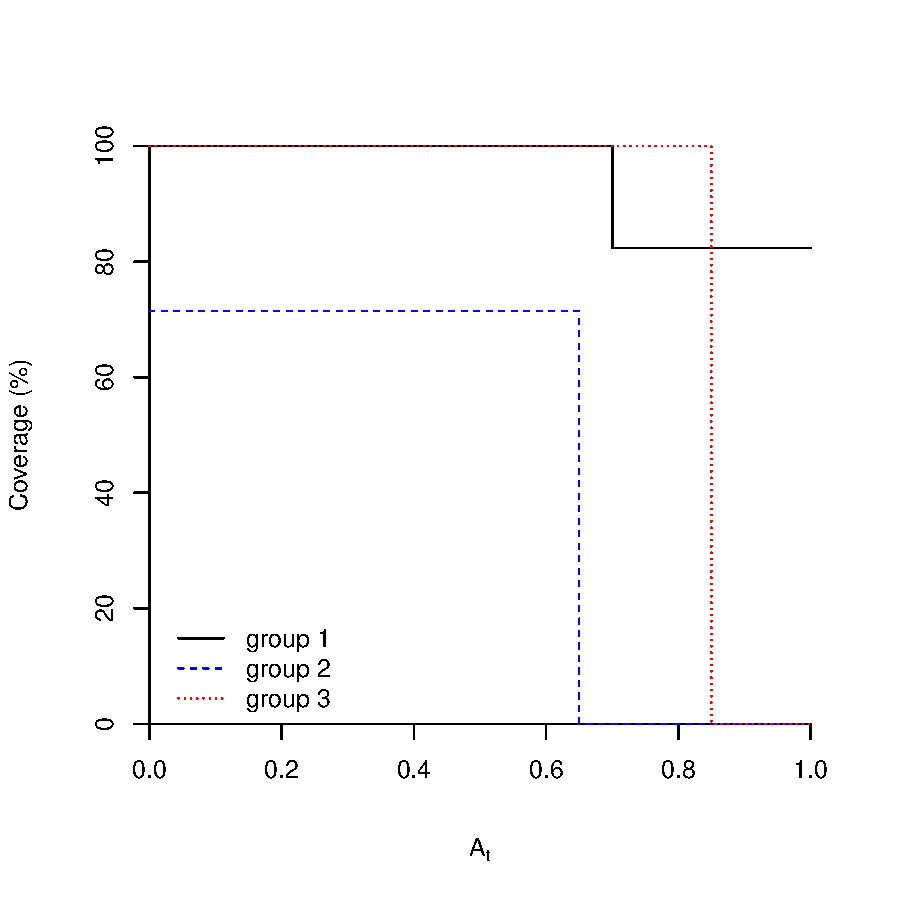
\includegraphics{indicspeciesTutorial-025}
\end{center}

As you can see in the example, function \texttt{plotcoverage} has to be called for one group at a time. However, several plots can be drawn one onto the other using the option \texttt{add=TRUE}.

\section{Species combinations as indicators of site groups}

Ecological indicators can be of many kinds. \citet{DeCaceres2012} recently explored the indicator value of \emph{combinations of species} instead of just considering individual species. The rationale behind this approach is that two or three species, when found together, bear more ecological information than a single one. 

\subsection{Generating species combinations}
The association between species combinations and groups of sites is studied in the same way as for individual species. However, instead of analyzing a site-by-species matrix, we need a matrix with as many rows as there are sites and as many columns as there are species combinations. We can obtain that matrix using the function \texttt{combinespecies}:
\begin{Schunk}
\begin{Sinput}
> wetcomb = combinespecies(wetland, max.order = 2)$XC
> dim(wetcomb)
\end{Sinput}
\begin{Soutput}
[1]  41 561
\end{Soutput}
\end{Schunk}
The resulting data frame has the same number of sites (i.e. 41) but as many columns as species combinations (in this case 561 columns). Each element of the data frame contains an abundance value, which is the minimum abundance value among all the species forming the combination, for the corresponding site. In our example, we used \texttt{max.order = 2} to limit the order of combinations. Therefore, only pairs of species were considered. Once we have this new data set, we can use it in \texttt{multipatt}:
\begin{Schunk}
\begin{Sinput}
> indvalspcomb = multipatt(wetcomb, groups, duleg = TRUE, 
+                        control = how(nperm=999))
> summary(indvalspcomb, indvalcomp = TRUE)
\end{Sinput}
\begin{Soutput}
 Multilevel pattern analysis
 ---------------------------

 Association function: IndVal.g
 Significance level (alpha): 0.05

 Total number of species: 561
 Selected number of species: 44 
 Number of species associated to 1 group: 44 
 Number of species associated to 2 groups: 0 

 List of species associated to each combination: 

 Group 1  #sps.  14 
                   A      B  stat p.value    
Ludads        1.0000 0.8235 0.907   0.001 ***
Orysp.+Ludads 1.0000 0.8235 0.907   0.001 ***
Orysp.        0.6772 1.0000 0.823   0.001 ***
Sessp.+Ludads 1.0000 0.4118 0.642   0.002 ** 
Orysp.+Psespi 1.0000 0.4118 0.642   0.007 ** 
Elesp.+Ludads 1.0000 0.4118 0.642   0.004 ** 
Psespi+Ludads 1.0000 0.4118 0.642   0.005 ** 
Orysp.+Elesp. 0.7424 0.5294 0.627   0.012 *  
Sessp.+Orysp. 0.9081 0.4118 0.611   0.010 ** 
Psespi        0.8811 0.4118 0.602   0.019 *  
Helind+Ludads 1.0000 0.3529 0.594   0.007 ** 
Walind+Orysp. 1.0000 0.2941 0.542   0.027 *  
Walind+Ludads 1.0000 0.2941 0.542   0.027 *  
Ipoaqu+Ludads 1.0000 0.2941 0.542   0.028 *  

 Group 2  #sps.  10 
                   A      B  stat p.value    
Phynod+Elesp. 0.9162 0.5714 0.724   0.001 ***
Phynod        0.6396 0.7143 0.676   0.008 ** 
Phynod+Helind 0.6922 0.6429 0.667   0.008 ** 
Helind+Elesp. 0.6861 0.5714 0.626   0.016 *  
Phynod+Echell 0.8654 0.3571 0.556   0.025 *  
Echell+Elesp. 0.8586 0.3571 0.554   0.015 *  
Melcor+Elesp. 0.7083 0.4286 0.551   0.047 *  
Aesind+Elesp. 1.0000 0.2857 0.535   0.017 *  
Echpas+Phynod 0.8293 0.2857 0.487   0.046 *  
Echpas+Cyprot 1.0000 0.2143 0.463   0.042 *  

 Group 3  #sps.  20 
                   A      B  stat p.value    
Pancam        0.8278 1.0000 0.910   0.001 ***
Pancam+Melcor 0.7769 1.0000 0.881   0.001 ***
Pancam+Echell 1.0000 0.6000 0.775   0.001 ***
Eupvac+Echell 1.0000 0.6000 0.775   0.001 ***
Pancam+Eupvac 0.7455 0.8000 0.772   0.001 ***
Melcor        0.5463 1.0000 0.739   0.001 ***
Melcor+Eupvac 0.6648 0.8000 0.729   0.001 ***
Eupvac        0.6546 0.8000 0.724   0.003 ** 
Pancam+Cynarc 1.0000 0.5000 0.707   0.001 ***
Pancam+Sessp. 0.8077 0.6000 0.696   0.003 ** 
Melcor+Echell 0.7368 0.6000 0.665   0.006 ** 
Melcor+Cynarc 0.8077 0.5000 0.635   0.003 ** 
Cynarc        0.7241 0.5000 0.602   0.013 *  
Melcor+Sessp. 0.5895 0.6000 0.595   0.032 *  
Eupvac+Cynarc 0.8485 0.4000 0.583   0.007 ** 
Cynarc+Sessp. 0.7778 0.4000 0.558   0.022 *  
Cynarc+Phynod 1.0000 0.3000 0.548   0.011 *  
Cynarc+Echell 1.0000 0.3000 0.548   0.010 ** 
Eupvac+Ipoaqu 1.0000 0.2000 0.447   0.042 *  
Cynarc+Ipoaqu 1.0000 0.2000 0.447   0.042 *  
---
Signif. codes:  0 '***' 0.001 '**' 0.01 '*' 0.05 '.' 0.1 ' ' 1 
\end{Soutput}
\end{Schunk}
The best indicators for both Group 1 and Group 3 are individual species (`Ludads' and `Pancam'). However, Group 2 is best indicated if we find, in the same community, `Phynod' and `Elesp'. Note that the species forming the indicator combination do not need to be good single-species indicators themselves. In our example `Phynod' is a good indicator of Group 2 but `Elesp.' is not.

\subsection{The function \texttt{indicators}}
In the previous example, there were many combinations of species that were significantly associated with site groups. There is another, more efficient, way of exploring the potential indicators for a given target site group. Say, for example, that we want to determine indicators for our Group 1, and we want to consider not only species pairs but also species trios. Since there are 33 species in the data set, the number of combinations can be very large. We can reduce the number of combinations to consider by selecting the \emph{candidate species} to combine. In this example, we choose those species whose frequency within Group 2 is larger than 20\%:
\begin{Schunk}
\begin{Sinput}
> B=strassoc(wetland, cluster=groups ,func="B") 
> sel=which(B[,2]>0.2) 
> sel
\end{Sinput}
\begin{Soutput}
 [1]  4  6  8  9 15 16 19 20 21 22 23 24 25 26
\end{Soutput}
\end{Schunk}
Object \texttt{sel} contains the indices of the 14 species that are candidates. Once we have our selection of candidate species, we can run the indicator analysis using:
\begin{Schunk}
\begin{Sinput}
> sc= indicators(X=wetland[,sel], cluster=groups, group=2, verbose=TRUE, 
+                At=0.5, Bt=0.2)
\end{Sinput}
\begin{Soutput}
Target site group: 2
Number of candidate species: 14
Number of sites: 41 
Size of the site group: 14 
Starting species  1 ... accepted combinations: 4 
Starting species  2 ... accepted combinations: 42 
Starting species  3 ... accepted combinations: 45 
Starting species  4 ... accepted combinations: 52 
Starting species  5 ... accepted combinations: 68 
Starting species  6 ... accepted combinations: 72 
Starting species  7 ... accepted combinations: 72 
Starting species  8 ... accepted combinations: 77 
Starting species  9 ... accepted combinations: 93 
Starting species  10 ... accepted combinations: 96 
Starting species  11 ... accepted combinations: 99 
Starting species  12 ... accepted combinations: 100 
Starting species  13 ... accepted combinations: 100 
Starting species  14 ... accepted combinations: 100 
Number of valid combinations: 100
Number of remaining species: 14 
\end{Soutput}
\end{Schunk}
We can discard species combinations with low indicator values by setting thresholds for components A and B (in our example using  \texttt{At=0.5} and \texttt{Bt=0.2}). The parameter \texttt{verbose = TRUE} allowed us to obtain information about the analysis process. Note that, by default, the \texttt{indicators} function will consider species combinations up to an order of 5. This can result in long computation times if the set of candidate species is not small. Similarly to \texttt{multipatt}, we can print the results of \texttt{indicators} for the most useful indicators, using:
\begin{Schunk}
\begin{Sinput}
> print(sc, sqrtIVt = 0.6)
\end{Sinput}
\begin{Soutput}
                                    A         B    sqrtIV
Phynod+Helind+Elesp.        1.0000000 0.5714286 0.7559289
Phynod+Elesp.               0.9000000 0.5714286 0.7171372
Phynod                      0.6666667 0.7142857 0.6900656
Phynod+Helind               0.7142857 0.6428571 0.6776309
Melcor+Phynod+Helind+Elesp. 1.0000000 0.4285714 0.6546537
Helind+Elesp.               0.6428571 0.5714286 0.6060915
Melcor+Phynod+Elesp.        0.8571429 0.4285714 0.6060915
Melcor+Helind+Elesp.        0.8571429 0.4285714 0.6060915
\end{Soutput}
\end{Schunk}
The species combinations are listed in decreasing indicator value order. In this case, we obtain that a combination of `Phynod', `Helind' and `Elesp.' is even a better indicator than `Phynod' and `Elesp.'. Note that the `A' and IndVal values for the pair `Phynod' and `Elesp.' do not exactly match those obtained before. This is because \texttt{indicators} uses `IndVal' and not `IndVal.g' as association statistic.

Although we did not show it here, \texttt{indicators} should in most cases be run with the option requesting for bootstrap confidence intervals (using option \texttt{nboot}), because they allow us to know the reliability of the indicator value estimates. This is specially important for site groups of small size \citep{DeCaceres2012}.

\subsection{Determining the coverage for objects of class \texttt{indicators}}
We can determine the proportion of sites of the target site group where one or another indicator is found, using, as shown before for objects of class \texttt{multipatt}, the function \texttt{coverage}:
\begin{Schunk}
\begin{Sinput}
> coverage(sc)
\end{Sinput}
\begin{Soutput}
[1] 1
\end{Soutput}
\end{Schunk}
In this case the coverage was complete (i.e. 100\%). Like we did for objects of class \texttt{multipatt}, we can add requirements to the validity of indicators. For example:
\begin{Schunk}
\begin{Sinput}
> coverage(sc, At=0.8)
\end{Sinput}
\begin{Soutput}
[1] 0.9285714
\end{Soutput}
\end{Schunk}
While we do not show here, in the case of objects of class \texttt{indicators} we recommend to explore the coverage using the lower boundary of confidence intervals, using option \texttt{type} of function \texttt{coverage}. 

Finally, we can also plot coverage values corresponding to different thresholds:
\begin{center}
\begin{Schunk}
\begin{Sinput}
> plotcoverage(sc)
> plotcoverage(sc, max.order=1, add=TRUE, lty=2, col="red")
> legend(x=0.1, y=20, legend=c("Species combinations","Species singletons"), 
+        lty=c(1,2), col=c("black","red"), bty="n")
\end{Sinput}
\end{Schunk}
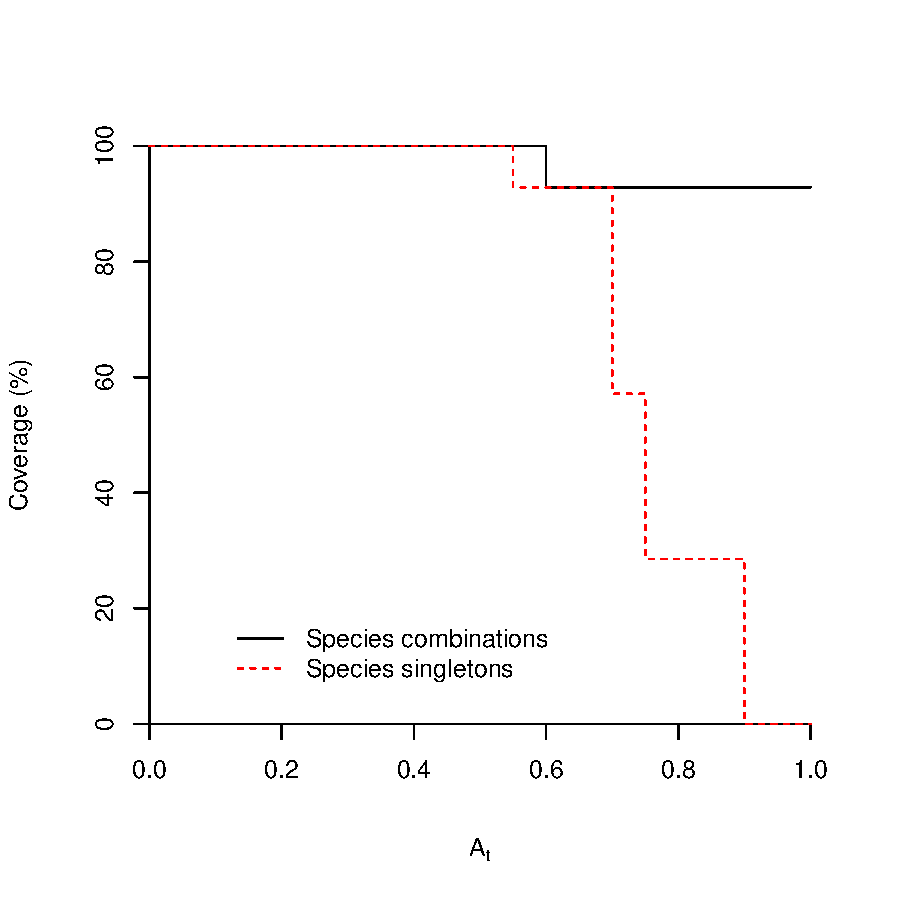
\includegraphics{indicspeciesTutorial-033}
\end{center}
The coverage plot tells us that if we want to use a very large `A' threshold (i.e., if we want to be very strict to select valid indicators), we won't have enough valid indicators to cover all the area of our target site group. This limitation is more severe if only single species are considered.

\subsection{The function \texttt{pruneindicators}}
As there may be many species combinations that could be used as indicators, the function \texttt{pruneindicators} helps us to reduce the possibilities. First, the function selects those indicators (species or species combinations) that are valid according to the input thresholds \texttt{At} and \texttt{Bt}. Second, the function discards those valid indicators whose occurrence patterns are nested within other valid indicators. Third, the function evaluates the coverage of the remaining set of indicators. Finally, it explores subsets of increasing number of indicators, until the same coverage as the coverage of the complete set is attained and the subset of indicators is returned.
\begin{Schunk}
\begin{Sinput}
> sc2=pruneindicators(sc, At=0.8, Bt=0.2, verbose=TRUE)
\end{Sinput}
\begin{Soutput}
Coverage of initial set of 100 indicators: 100%
Coverage of valid set of 52 indicators: 92.9%
Coverage of valid set of 7 nonnested indicators: 92.9%
Checking 7 subsets of 1 indicator(s) maximum coverage: 57.1%
Checking 21 subsets of 2 indicator(s).......... maximum coverage: 85.7%
Checking 35 subsets of 3 indicator(s)........ maximum coverage: 92.9%
Coverage of final set of 3 indicators: 92.9%
\end{Soutput}
\begin{Sinput}
> print(sc2)
\end{Sinput}
\begin{Soutput}
                      A         B    sqrtIV
Phynod+Elesp. 0.9000000 0.5714286 0.7171372
Cyprot        0.8666667 0.2857143 0.4976134
Echpas+Phynod 0.8000000 0.2857143 0.4780914
\end{Soutput}
\end{Schunk}
In our example, and using these thresholds, the best indicators would be: (1) the combination of `Phynod' and `Elesp.'; (2) `Cyprot' and (3) `Echpas' and `Phynod'. The three indicators together cover 93\% of the sites belonging to the target site group.

\subsection{The function \texttt{predict.indicators}}
The function \texttt{indicators} provides a model that can be used to predict a target site group. Once a given combination of species has been found, the corresponding \texttt{A} value is the probability of being in the target site group given the combination of species has been found. Therefore, the set of indicators could be used to predict the likelihood of the target site group in a new data set. The function \texttt{predict.indicators} has exactly this role. It takes the results of \texttt{indicators} and a new community data matrix as input. Given this input, the function calculates the probability of the target site group for each site. The following code exemplifies the use of \texttt{predict.indicators} with the same data that was used for the calibration of the indicator model (a new community data matrix should be used in normal applications):
\begin{Schunk}
\begin{Sinput}
> p<-predict(sc2, wetland)
\end{Sinput}
\end{Schunk}
Of course, this will return biased estimates, as the data set used to build the model is the same as the target data set for which probabilities are desired. The same would be obtained using:
\begin{Schunk}
\begin{Sinput}
> p<-predict(sc2)
\end{Sinput}
\end{Schunk}
which uses the original data set storied in the \texttt{indicators} object. If we want to evaluate these probabilities in a cross-validated fashion (i.e., excluding each target site for the calculation of positive predictive values and the probability of the target site group), we can use:
\begin{Schunk}
\begin{Sinput}
> pcv<-predict(sc2, cv=TRUE)
\end{Sinput}
\end{Schunk}
We can compare the probabilities (evaluated by resubstitution and cross-validation) with the original group memberships:
\begin{Schunk}
\begin{Sinput}
> data.frame(Group1 = as.numeric(wetkm$cluster==1), Prob = p, Prob_CV = pcv)
\end{Sinput}
\begin{Soutput}
   Group1      Prob   Prob_CV
5       0 0.0000000 0.0000000
8       0 0.0000000 0.0000000
13      0 0.0000000 0.0000000
4       0 0.0000000 0.0000000
17      0 0.0000000 0.0000000
3       0 0.0000000 0.0000000
9       0 0.0000000 0.0000000
21      0 0.0000000 0.0000000
16      0 0.0000000 0.0000000
14      0 0.0000000 0.0000000
2       0 0.0000000 0.0000000
15      0 0.0000000 0.0000000
1       0 0.0000000 0.0000000
7       0 0.0000000 0.0000000
10      0 0.0000000 0.0000000
40      1 0.9000000 1.0000000
23      1 0.0000000 0.0000000
25      1 0.9000000 0.8888889
22      0 0.8000000 0.7500000
20      1 0.9000000 0.8888889
6       1 0.9000000 0.8888889
18      1 0.9000000 0.8888889
12      1 0.9000000 0.8888889
39      1 0.9000000 0.8888889
19      1 0.9000000 0.8750000
11      1 0.9000000 0.8888889
30      1 0.8666667 0.8181818
34      1 0.8666667 0.8333333
28      1 0.0000000 0.0000000
31      1 0.8666667 0.8461538
26      1 0.8666667 0.8181818
29      1 0.8666667 0.9285714
33      1 0.8666667 0.9285714
24      1 0.0000000 0.0000000
36      1 0.0000000 0.0000000
37      1 0.0000000 0.0000000
41      1 0.0000000 0.0000000
27      1 0.0000000 0.0000000
32      1 0.0000000 0.0000000
35      0 0.0000000 0.0000000
38      0 0.0000000 0.0000000
\end{Soutput}
\end{Schunk}
Cross-validated probabilities will tend to be lower than probabilities evaluated by resubstitution for sites originally belonging to the target site group and higher for other sites.
\bibliographystyle{plainnat}
\bibliography{indicspecies}
\end{document}
